\documentclass[twoside,twocolumn]{article}

\usepackage{blindtext} % Package to generate dummy text throughout this template 
\usepackage{graphicx}
\usepackage[sc]{mathpazo} % Use the Palatino font
\usepackage[T1]{fontenc} % Use 8-bit encoding that has 256 glyphs
\linespread{1.05} % Line spacing - Palatino needs more space between lines
\usepackage{microtype} % Slightly tweak font spacing for aesthetics

\usepackage[english]{babel} % Language hyphenation and typographical rules

\usepackage[hmarginratio=1:1,top=32mm,columnsep=20pt]{geometry} % Document margins
\usepackage[hang, small,labelfont=bf,up,textfont=it,up]{caption} % Custom captions under/above floats in tables or figures
\usepackage{booktabs} % Horizontal rules in tables
\usepackage{graphicx}
\usepackage{lettrine} % The lettrine is the first enlarged letter at the beginning of the text

\usepackage{enumitem} % Customized lists
\setlist[itemize]{noitemsep} % Make itemize lists more compact

\usepackage{abstract} % Allows abstract customization
\renewcommand{\abstractnamefont}{\normalfont\bfseries} % Set the "Abstract" text to bold
\renewcommand{\abstracttextfont}{\normalfont\small\itshape} % Set the abstract itself to small italic text

\usepackage{titlesec} % Allows customization of titles
\renewcommand\thesection{\Roman{section}} % Roman numerals for the sections
\renewcommand\thesubsection{\roman{subsection}} % roman numerals for subsections
\titleformat{\section}[block]{\large\scshape\centering}{\thesection.}{1em}{} % Change the look of the section titles
\titleformat{\subsection}[block]{\large}{\thesubsection.}{1em}{} % Change the look of the section titles

\usepackage{fancyhdr} % Headers and footers
\pagestyle{fancy} % All pages have headers and footers
\fancyhead{} % Blank out the default header
\fancyfoot{} % Blank out the default footer
\fancyhead[C]{Patrones de diseño $\bullet$ Octubre 2020 $\bullet$ } % Custom header text
\fancyfoot[RO,LE]{\thepage} % Custom footer text

\usepackage{titling} % Customizing the title section

\usepackage{hyperref} % For hyperlinks in the PDF

%----------------------------------------------------------------------------------------
%	TITLE SECTION
%----------------------------------------------------------------------------------------

\setlength{\droptitle}{-4\baselineskip} % Move the title up

\pretitle{\begin{center}\Huge\bfseries} % Article title formatting
\posttitle{\end{center}} % Article title closing formatting
\title{Patrones de diseño} % Article title
\author{Derian Herrera, Julio Mejia, Randi Paredes , Marco Garcia y Alisson Chino}
\date{\today} % Leave empty to omit a date
\renewcommand{\maketitlehookd}{%

}

%----------------------------------------------------------------------------------------

\begin{document}

% Print the title
\maketitle

%----------------------------------------------------------------------------------------
%	ARTICLE CONTENTS
%----------------------------------------------------------------------------------------

\section{Resumen}

\lettrine[nindent=0em,lines=3]{E}n el siguiente articulo observaremos algunos
de los patrones de diseño usados.
Los diseñadores  expertos no solucionan los problemas desde  sus principios
sino que reutilizan soluciones  que anteriormente funcionaron.
Aqui se encuentran los patrones de diseño que resuelven problemas especificos 
y hacen el diseño flexible  y reusable.



%------------------------------------------------

\section{Abstract}


In the following article we will observe some
of the design patterns used.
Expert designers do not solve problems from the beginning
instead they reuse solutions that previously worked.
Here are the design patterns that solve specific problems
and they make the design flexible and reusable.





%------------------------------------------------
\section{Introduccion}
Los patrones de diseño es un tema  importante  en el desarrollo  de software 
actual, lo que busca es ayudar  a los desarrolladores de software a resolver  problemas comunes
creando un lenguaje comun  para comunicar ideas  y experiencias acerca de problemas 
y soluciones.
El usar patrones de diseño ayuda a tener un software de calidad.
Según su proposito  los patrones se pueden clasificar en tres:
De creacion, proceso de creacion de objetos.
De estructura, tratan composicion de clases y/o objetos.
De comportamiento, se caracterizan en la forma que interactuan y reparten responsabilidades
 a sus clases y objetos.

\section{Desarrollo}

\subsection{Patron de diseño observer}

El patron de diseño observer es un patron comportamental,este patron define 
una dependencia de uno a muchos entre objetos, de forma que cuando un objeto 
cambie de estado se notifique y se actualicen automáticamente todos los
 objetos que depende de él.
 \begin{itemize}
 \item  \textbf{Descripcion}
 \\ {- Los objetos principales son "Subject" y "Observer"}
 \\ {- La motivacion de este patron es la reutilizacion}
 \\ {- Puede no haber relacion directa entre objetos}
 \\ {- El tipo de interaccion es conocida como publicar-suscribir}
 \\ {- El subject es publicador de notificaciones}
 \\ {- Cualquier numero de observers puede suscribirse para recibir notificaiones}
\\
\\
 \item  \textbf{Componentes}
 \\ \textbf{Subject}
 \\Cualquier numero de observers puede observar a subject
 \\ \textbf{Observer}
 \\Define  una interfaz de actualizacion para los objetos Observer que deben ser notificados de los cambios en el Subject
 \\ \textbf{Concrete Subject}
 \\Almacena estados de interes  para  los objetos Concrete Observer.
 \\Envia notificaciones a sus observers cuando el estado cambia.
\\ \textbf{Concrete Observer}
\\Mantiene referencia  de objetos Concrete Subject.
\\Almacena los estados que deben ser consistentes con los subjects.
\\Implementa las observaciones del observer.
\\
\\
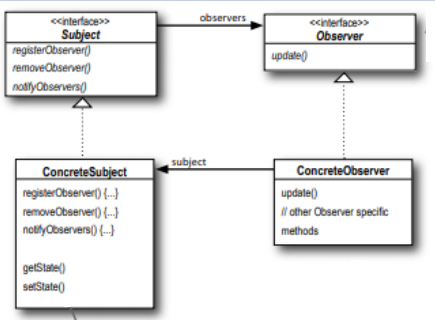
\includegraphics[width=7cm, height=6cm]{imagenes/observer.png}
\\
\item  \textbf{Ventajas}
\\-Permite  variar los sujetos y observadores indepedientemente.Se puede
rehusar sujetos  sin el rehuso de observadores  y viceversa.
\\-Permite agregar observadores sin modificar el sujeto o los observadores.
\item  \textbf{Desventajas}
\\-No se especifica  el receptor de una actualizacion.Se envia a todos los objetos interesados.
\\-Actualizaciones inesperadas.Se podrian dar actualizaciones en casacada muy ineficientes.

\item  \textbf{Ejemplo}
\\Crearemos un ejemplo en el cual al ingresar un monto en soles el programa
 nos dara la alerta segun el observador de cuando sera el cambio a la moneda de 
 ese observador.

\end{itemize}



 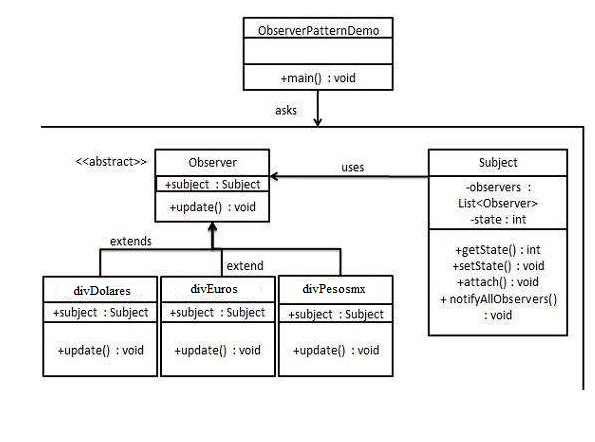
\includegraphics[width=7cm, height=7cm]{imagenes/observerEj.png}
 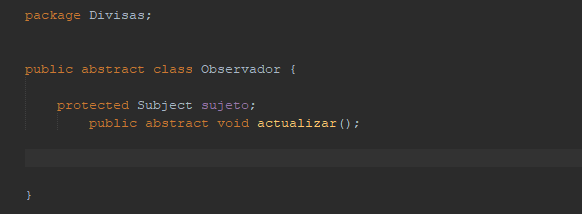
\includegraphics[width=7cm, height=6cm]{imagenes/eje1.png}
 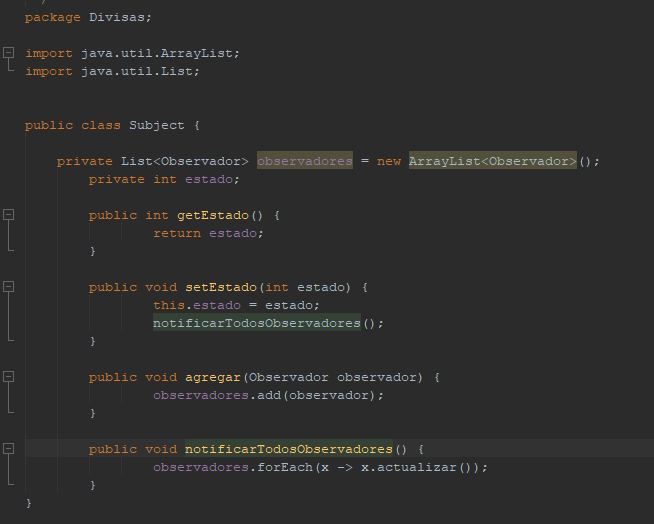
\includegraphics[width=7cm, height=6cm]{imagenes/eje2.png}
 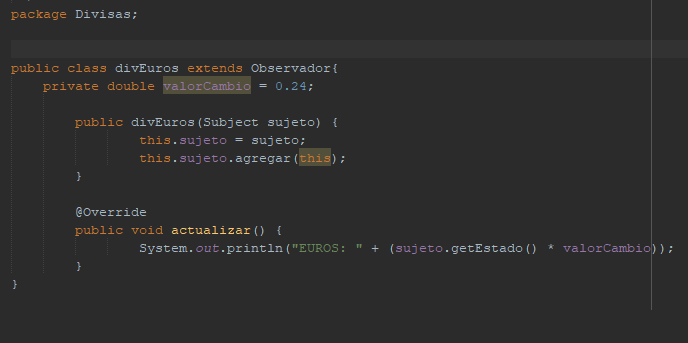
\includegraphics[width=7cm, height=6cm]{imagenes/eje3.png}
 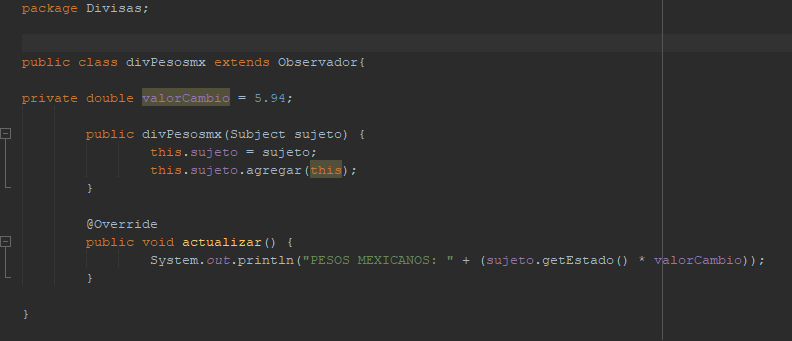
\includegraphics[width=7cm, height=6cm]{imagenes/eje4.png}


\subsection{Patron Facade}
Proporcionar una interfaz unificada a un conjunto de interfaces en un subsistema. Facade define una interfaz de nivel superior que facilita el uso del subsistema.
\\
Las fachadas se pueden utilizar no solo para crear una interfaz más simple en términos
de llamadas a métodos, sino también para reducir el número de objetos que un cliente
objeto debe tratar. Facade es un patrón de diseño de software que se usa comúnmente en la programación orientada a objetos. Facade es un objeto que sirve como una interfaz frontal que enmascara un código estructural o subyacente más complejo.
\\
Los desarrolladores suelen utilizar el patrón de diseño Facade cuando un sistema es muy complejo o difícil de entender porque el sistema tiene muchas clases interdependientes o porque su código fuente no está disponible. Este patrón oculta las complejidades del sistema más grande y proporciona una interfaz más simple para el cliente. Por lo general, involucra una sola clase contenedora que contiene un conjunto de miembros requeridos por el cliente. Estos miembros acceden al sistema en nombre del cliente de fachada y ocultan los detalles de implementación.
\\

\begin{itemize}

\item  \textbf{Caracteristicas}
\\
\\ \textbf{Intención}
Quiere simplificar cómo utilizar un sistema existente. Necesitas definir
su propia interfaz.
\\ \textbf{Problema}
Necesita utilizar solo un subconjunto de un sistema complejo. O necesita interactuar con el sistema de una manera particular.
\\ \textbf{Solución}
Facade presenta una nueva interfaz para que la utilice el cliente del sistema existente.
\\ \textbf{Participantes}
Facade presenta una nueva interfaz para que la utilice el cliente del sistema existente.
\\ \textbf{Consecuencias}
Facade simplifica el uso del subsistema requerido. Sin embargo, debido a que la fachada no está completa, es posible que el cliente no disponga de determinadas funciones.
\\ \textbf{Implementación}
Defina una nueva clase (o clases) que tenga la interfaz requerida.
\\
\item  \textbf{Ventajas}
Una de las ventajas de utilizar este patrón a la hora de controlar los permisos de los usuarios, es que cada usuario tiene un rol (administrador, invitado, usuario registrado, etc.)
La principal ventaja del patrón Facade consiste en que para modificar las clases de los subsistemas, sólo hay que realizar cambios en la interfaz / fachada, y los clientes pueden permanecer ajenos a ello. Además, y como se mencionó anteriormente, los clientes no necesitan conocer las clases que hay tras dicha interfaz.

\item  \textbf{Desventajas}
Como inconveniente, si se considera el caso de que varios clientes necesiten acceder a subconjuntos diferentes de la función que proporcionan el sistema, podrían acabar usando sólo una pequeña parte de la fachada, por lo que sería conveniente utilizar varias fachadas más específicas en el lugar de una única global.
Oculta a los clientes los componentes del subsistema, reduciendo así el número de objetos con los que tratan los clientes y haciendo que el subsistema sea más fácil de usar.
\item  \textbf{Ejemplo}

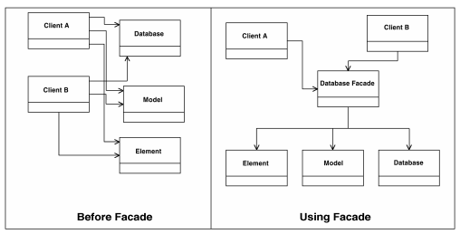
\includegraphics[width=6cm, height=4cm]{imagenes/facade.png}
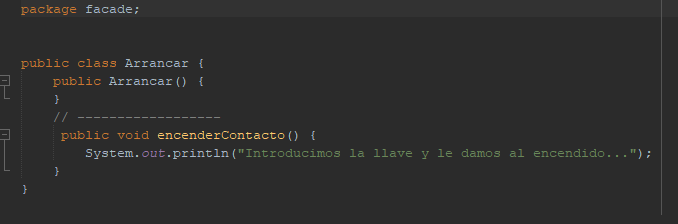
\includegraphics[width=6cm, height=4cm]{imagenes/faca1.png}
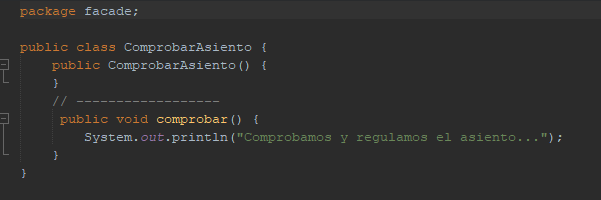
\includegraphics[width=6cm, height=4cm]{imagenes/faca2.png}
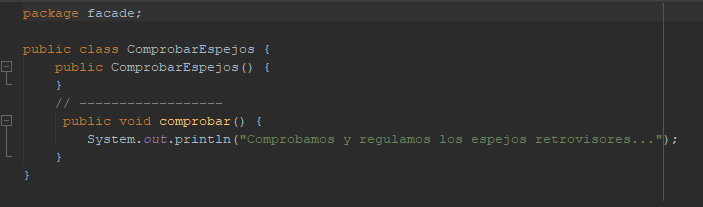
\includegraphics[width=6cm, height=4cm]{imagenes/faca3.png}
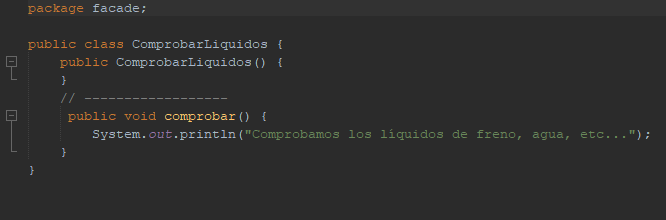
\includegraphics[width=6cm, height=4cm]{imagenes/faca4.png}
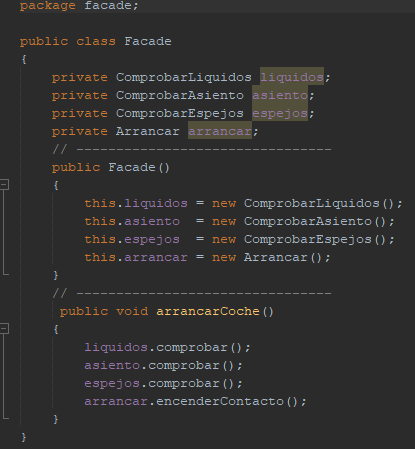
\includegraphics[width=6cm, height=4cm]{imagenes/faca5.png}
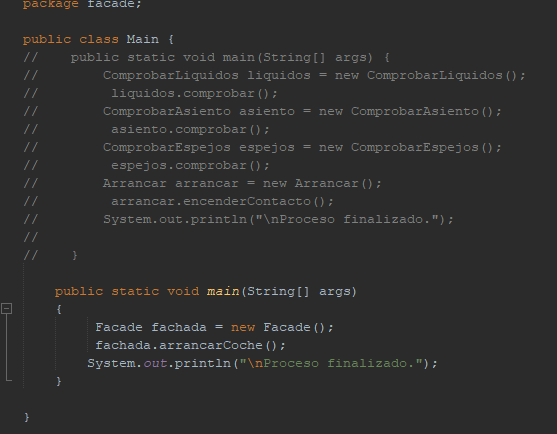
\includegraphics[width=6cm, height=4cm]{imagenes/faca6.png}



\end{itemize}

\subsection{Patrón de Diseño: FACTORY}
El patrón de diseño Factory nos permite la creación de un subtipo determinado por medio de una clase de Factory, la cual oculta los detalles de creación del objeto.
El objeto creado es enmascarado detrás de una interfaz común entre todos los objetos que pueden ser creado, con la finalidad de que estos pueden variar sin afectar la forma en que el cliente interactúa con ellos. 

En un Factory es normal que pueda crear varios subtipos de una determinada interfaz y que todos los objetos concretos fabricados hagan una tarea similar, pero con detalles de implementación diferentes. La intención 
del Factory es tener una clase a la cual delegar la responsabilidad de la creación de los objetos, para que no sea el mismo programador el que decida que clase es la que instanciará, si no que delegará esta responsabilidad 
al Factory confiando en que este le regresará la clase adecuada para trabajar.


\begin{itemize}

\item  \textbf{ESTRUCTURA}  

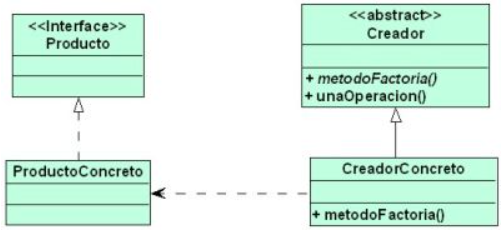
\includegraphics[width=7cm, height=7cm]{imagenes/Factoryp.png}
\textbf{Productos Abstractos}
son los que declaran interfaces para un grupo de productos diferentes pero relacionados que forman una familia de productos.
\\
\\\textbf{Productos Concretos}
son implementaciones distintas de productos abstractos agrupados por variantes. Cada producto abstracto (silla/sofá) debe implementarse en todas las variantes dadas (victoriano/moderno).
\\
\\\textbf{Fábrica Abstracta }
en esa interfaz se declara un grupo de métodos para crear cada uno de los productos abstractos.
\\
\\\textbf{Fábricas Concretas}
implementan métodos de creación de la fábrica abstracta. Cada fábrica concreta se corresponde con una variante específica de los productos y crea tan solo dichas variantes de los productos.
\\\item  \textbf{VENTAJAS}
\\ La ventaja de usar este patrón es que elimina la necesidad de instanciar los objetos de forma explicita que se utilizaran, también nos permitirá encapsular en las clases Factory la lógica de creación de los objetos, que incluso pueden ser mas complejas que realizar el (new).
Es extensible ya que la arquitectura queda libre a desarrollos con nuevas clases que extienden a Factory y la familia de productos, también de esa manera responde al principio SOLID de open/close.
\\\item  \textbf{DESVENTAJAS}
\\ La desventaja es ya que Factory se usará para crear objetos que heredan una clase en común, puede que sea necesario mucho código repetitivo en cada una de las subclases.
También al delegar funciones puede ser mas complejo encontrar en primera instancia la mecánica de funcionamiento del sistema. 
Al momento de querer añadir un nuevo producto, se necesita la implementación de la interfaz y todos sus métodos.
\\\item  \textbf{EJEMPLO}
\\
\\
\\- Creamos dos clases de tipo IArchivo así como la clase abstracta en la que se define el método de fabricación, y otra que hereda de ella y lo implementa.
\\- En el programa principal se crea una instancia de la clase que implementa el método de fabricación, el cual usaremos para crear y devolver los distintos tipos de objetos.
\\  
\\Main.java
\\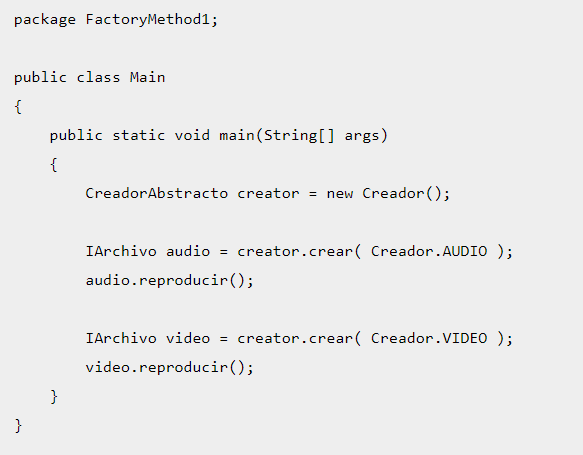
\includegraphics[width=7cm, height=6cm]{imagenes/Cod.png}
\\IArchivo.java
\\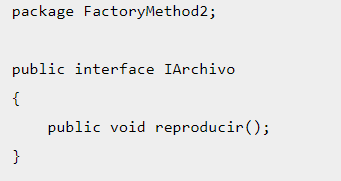
\includegraphics[width=7cm, height=6cm]{imagenes/cod2.png}
\\Creador.java 
\\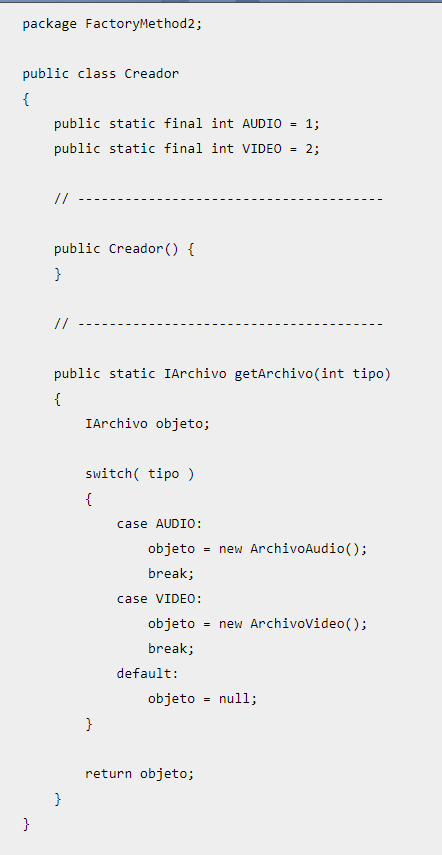
\includegraphics[width=7cm, height=6cm]{imagenes/Cod3.png}
\\CreadorAbstracto.java
\\\includegraphics[width=7cm, height=6cm]{imagenes/Cod4.png}

\section{Conclusiones}
{- Conocer los patrones de diseño facilita la comprensión de los sistemas existentes.}
\\
\\{- Las personas que aprenden programación orientada a objetos a menudo se quejan de que los sistemas con los que están trabajando usan la herencia de formas complicadas y que es difícil seguir el flujo de control. En gran parte, esto se debe a que no comprenden los patrones de diseño del sistema. Aprender estos patrones de diseño lo ayudará a comprender los sistemas orientados a objetos existentes.}
\\
\\{- Estos patrones de diseño también pueden convertirlo en un mejor diseñador. }
\\
\\{- Proporcionan soluciones a problemas comunes. Si trabaja con sistemas orientados a objetos el tiempo suficiente, probablemente aprenderá estos patrones de diseño por su cuenta. Aprender estos patrones ayudará a un novato a actuar más como un experto.}
\\
\\{- Además, describir un sistema en términos de los patrones de diseño que utiliza hará que sea mucho más fácil de entender. De lo contrario, la gente tendrá que realizar ingeniería inversa en el diseño para descubrir los patrones que utiliza}
\\
\\{- Tener un vocabulario común significa que no tiene que describir todo el patrón de diseño; puede simplemente nombrarlo y esperar que su lector lo sepa. Un lector que no conozca los patrones tendrá que buscarlos al principio, pero eso sigue siendo más fácil que la ingeniería inversa.}

\end{itemize}
\section{Recomendaciones}
%----------------------------------------------------------------------------------------
%	REFERENCE LIST
%----------------------------------------------------------------------------------------
Como recomendacion usar un patron de diseño es algo que el programador
debe elegir ya que cada patron se acomoda a soluciones a diferentes problemas 
, por eso existen distintos tipos de patrones los cuales el desarrollador puede usar y
 asi ahorrarse tiempo escencial para el desarrollo de software.
\begin{thebibliography}{99} % Bibliography - this is intentionally simple in this template

\bibitem
.Elisabeth Freeman, Kathy Sierra (2004).
\newblock Head First design patterns,
\newblock Sebastopol,
\newblock CA: O'Reilly.
\bibitem
.Scott Millett, Nick Tune (2015).
\newblock Patterns, Principles and Practices of Domain-Driven Design,
vvvvvvvvv
\bibitem
.Bipin Joshi (2004).
\newblock Beginning SOLID Principles and Design Patterns for ASP.NET Developers,
\newblock Sebastopol,
\newblock CA: O'Reilly.

\bibitem .Holzner
\newblock S., 2006. Design Patterns For Dummies. Hoboken, N.J.: Wiley.
 
\bibitem .Oscar Belmonte 
\newblock , Carlos Granell, Maria del Carmen Erdozain.(2012).
\newblock Desarrollo de proyectos informaticos con teconologia java. Universitat jaumen I
 
\end{thebibliography}

%----------------------------------------------------------------------------------------

\end{document}